\chapter{Analytical Calculations}
\label{sec:analytical}
\newcommand{\ta}{\ensuremath{\tilde \alpha}}
In ref. \cite{khodas}, Khodas et.~al. write about the effects of an
interface between regions of different strengths of Rashba spin-orbit
coupling. We take up their approach and expand on it.

Note that
we use a coordinate system here which differs from the one used in the
rest of this thesis. In particular, we assume the 2DEG in the $x-z$
plane (instead of $x-y$ plane), both for consistency with
ref. \cite{khodas} and because it makes the spinors real vectors and
thus simpler to handle. The results for the $T$ matrix in the end are
the same in both coordinate systems.

\section{Interface Between Normal and Spin-Orbit Coupling Regions}

\begin{figure}
    \begin{center}
        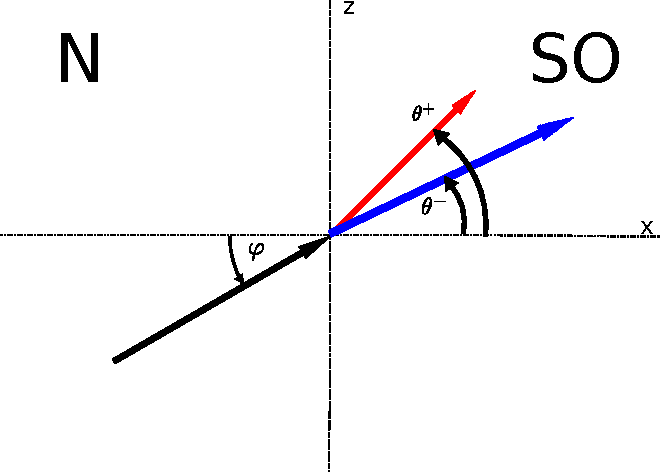
\includegraphics{setup-simple.pdf}
    \end{center}
    \caption{Scheme of the interface between normal (N)
            and spin-orbit (SO) regime}
    \label{fig:setup-zero}
\end{figure}

The setup consists of a 2D electron gas in the $x-z$ plane, where the
strength of the spin orbit interaction is a step function in $x$:
$\alpha(x) = \alpha \Theta(x)$. The region $x < 0$ is called the
"normal region", abbreviated with N, and the region with $x > 0$ is
called the "spin orbit" region, abbreviated as SO (Fig.
\ref{fig:setup-zero}).


The Hamiltonian looks like this:

\begin{align}
    H_r &= \frac{p^2}{2m} + (-\vec y \times \vec \sigma) \cdot
            \alpha(x) \vec p\\ 
    p^2 &= p_x^2 + p_z^2
\end{align}

with the eigenvalues and the velocities

\begin{align}
    E_{\pm} &= \frac{p^2}{2m} \pm \alpha \\
    v_{\pm} &= \frac{\partial E_{\pm}}{\partial p} = \frac{p}{m} \pm \alpha
\end{align}

When a wave travels from the N to the SO region, its energy does not
change. Since its dispersion relation changes, the momentum must also
change. From here on, when we write $p$ we mean the momentum in the N
region. The momentum in the SO region then follows as

\begin{align}
    \label{eq:pso}
    p_{SO}^{\pm} &= m v_F (\sqrt{1 + \ta^2} \mp \tilde \alpha) \\
    \tilde\alpha &= \frac{\alpha}{v_F}
\end{align}

$p_z$ is conserved at the interface.

Since $p_{SO}^+ \not = P_{SO}^-$ for $\ta \not = 0$, we see that
the beam splits up at the interface into two beams of opposite
chiralities and different angles $\theta^+$ and $\theta^-$.

The split up of the beams is approximately proportional to $\ta$:

\begin{align}
    \theta^+ - \theta^- = 2 \ta \tan \phi + O(\ta^3)
\end{align}

Solving the eigenvalue equation leads us to the eigenvectors in the SO
region:

\begin{align}
   \chi_{SO}^{\pm} &= \frac{1}{n_{SO}^{\pm}} 
                      \vect{-p_{x,SO}^{\pm} \pm p_{SO}^\pm}{p_z} \\
    n_{SO}^{\pm}   &= \sqrt{|-p_{x,SO}^{\pm} \pm p_{SO}^\pm|^2 +
        p_z^2}
    \label{eq:chi-so-pm}
\end{align}

where the lower index $x$ means that the value is projected onto the
$x$ axis. The angle between the $x$ axis and the momentum of the
incident wave is called $\phi$, so that $p_x = p \cos \phi$.

If one wants to expand $\chi_{SO}^\pm$ in powers of $\ta$, it is
important to ensure that the normalization condition
$\chi_{SO}^{\pm\dagger} \cdot \chi_{SO}^\pm$ still holds after the
expansion. However, the following results have been derived for the
full (and not expanded) form of $\chi_{SO}^\pm$.

Note that, in the N regime, $H$ is a diagonal matrix, and the direction
of the eigenvectors can be chosen with some freedom. We pick
$\chi_N^{\pm} = \lim_{\ta \mapsto 0} \chi_{SO}^{\pm}$ to ensure that
$<\chi_N^+|\chi_{SO}^+> = 1$ holds true at a vanishing interface.

\begin{align}
   \chi_N^{\pm} &= \frac{1}{n^{\pm}} 
                      \vect{-p_x \pm p}{p_z} \\
    n^{\pm} &= \sqrt{(-p_x \pm p)^2 + p_z^2}
\end{align}


The overall wave function consists of an incident wave, 
reflected and transmitted part. In general, the incident wave can
be decomposed into one with $+$ and one with $-$ chirality, which
propagate and scatter independently. Let us consider the incident $+$
wave:

\begin{align}
    \Psi^+ = e^{i p_z z} * \left\{
        \begin{array}{ll}
            e^{i p_x x} \chi_N^+ + e^{- i p_x x} (\chi_N^+ r_{++} +
                    \chi_N^- r_{-+})    & x < 0\\
            e^{i p_x^+ x} \chi_{SO}^+ t_{++} + e^{i p_x^- x}
            \chi_{SO}^- t_{-+}          & x > 0
        \end{array} \right.
        \label{eq:chiral-wafe-function}
\end{align}

The coefficient $r_{-+}$ is the amplitude with which the incident wave
of $+$ chirality is reflected into $-$ chirality etc., while $t$
coefficients stand for transmission coefficients.

Analog equations can be found for the incident wave with $-$ chirality
by changing all signs that appear either as a subscript or
superscript.

To obtain the values for these coefficients, one has to solve the
boundary conditions at the interface. The wave function is continuous
and the current is conserved, so $\frac{\partial H}{\partial p_x} \Psi$ is also
continuous:

\begin{align}
    \Psi_N|_{x = -0}    &= \Psi_{SO}|_{x = +0} \label{eq:continuous}\\
    \left.\frac{\hat p_x}{m} \Psi_N\right|_{x = -0}
                        &= \left. \left(\frac{\hat p_x}{m} -\alpha \sigma_z\right)
                                \Psi_{SO}\right|_{x = +0}
\end{align}

The second equation can be evaluated with $\hat p_x = -i \partial_x$
(assuming $\hbar = 1$, as done in the rest of the calculation).
Carrying out the derivative (and multiplying by $m$) yields:

\begin{align}
    p_x \chi_N^+ (1 - r_{++}) - p_x \chi_N^- r_{-+}
        =& p_x^+ \chi_{SO}^+ t_{++} + p_x^- \chi_{SO}^- t_{-+} \nonumber\\
         &   - m \alpha \left(  \sigma_z \chi_{SO}^+ t_{++}
                            + \sigma_z \chi_{SO}^- t_{-+} \right)
\end{align}

and dived by  $p_x = p \cos \phi$: 

\begin{align}
    \chi_N^+ (1 - r_{++}) - \chi_N^- r_{-+}
        =& \frac{p_x^+}{p_x} \chi_{SO}^+ t_{++} + \frac{p_x^-}{p_x} \chi_{SO}^- t_{-+} \nonumber\\
         &   - \frac{\ta}{\cos \phi} \left(\sigma_z \chi_{SO}^+
                 t_{++} + \sigma_z \chi_{SO}^- t_{-+} \right)
                                \label{eq:j_continuous}
\end{align}

Equations \ref{eq:continuous} and \ref{eq:j_continuous} have two
components each and can be solved unambiguously. 
The solutions expanded to the first non-zero order in $\ta$ each are

\begin{align}
    t_{++} &= 1 +
            \frac{\ta}{2}\left( \frac{1}{\cos^2\phi} - 1 \right)\\
    t_{-+} &= O(\ta^3)\\
    r_{++} &= \frac{\ta}{2} \tan^2 \phi\\
    r_{-+} &= -\frac{\ta}{2} \tan \phi
\end{align}

and for the incident wave with $-$ chirality

\begin{align}
    t_{--} &= 1 - \frac{\ta}{2} \left( \frac{1}{\cos^2\phi} - 1 \right)\\
    t_{+-} &= O(\ta^3)\\
    r_{--} &= -\frac{\ta}{2} \tan^2 \phi\\
    r_{+-} &= -\frac{\ta}{2} \tan \phi
\end{align}

\begin{figure}[h!tp]
    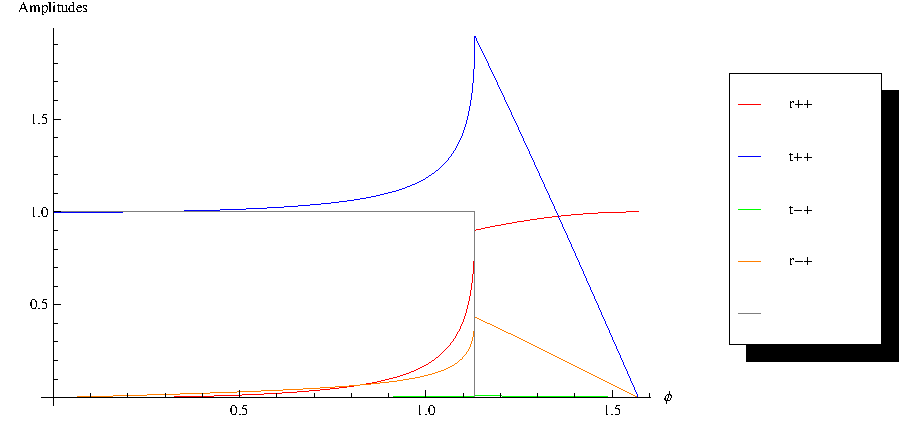
\includegraphics[width=\textwidth]{zero-plus.pdf}
    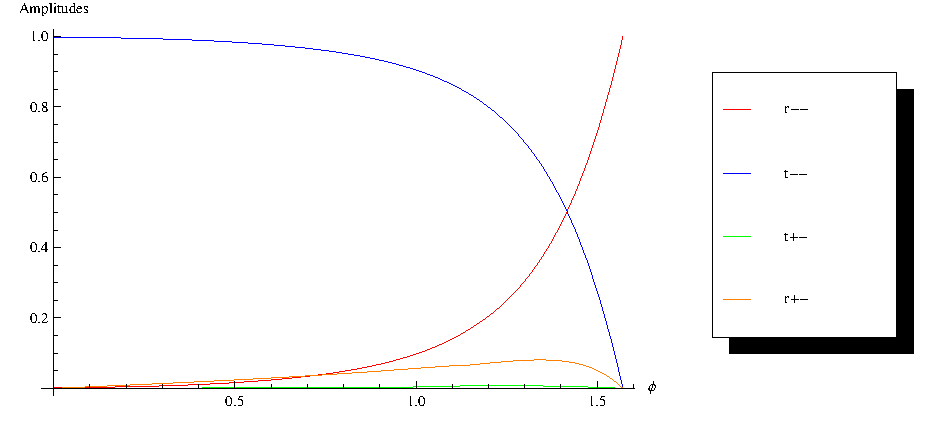
\includegraphics[width=\textwidth]{zero-minus.pdf}
    \caption{Transmission and reflection coefficients for the
            incident beam with $+$ (upper) and $-$ (lower) chirality
            and $\ta = 0.1$}
    \label{fig:trans-zero}
\end{figure}

Figure \ref{fig:trans-zero} shows the transmission and reflection
coefficients as a function of the angle $\phi$ of the incident wave.

For increasing $\phi$, the angle of the transmitted beam with $+$
chirality, $\theta^+$, grows even faster. When $\theta^+ >=
\frac{\pi}{2}$, the momentum $p_{x,SO}^+$ is imaginary and no current flows
anymore with $+$ chirality. 

\begin{figure}[tbh]
    \begin{center}
        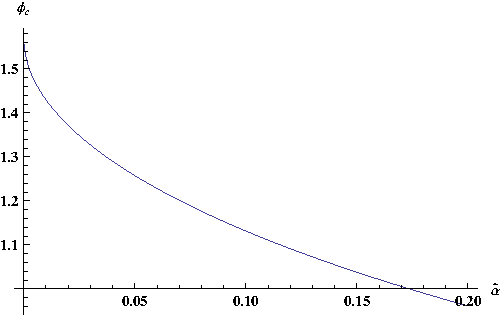
\includegraphics[width=0.7\textwidth]{critical-angle.pdf}
    \end{center}
    \caption{Critical angle $\phi_c$ as a function of $\ta$. For $\phi
        > \phi_c$ the wave associated with $t_{++}$ is evanescent.}
    \label{fig:critical-angle}
\end{figure}

The angle $\phi$ for which $\theta^+ =\frac{\pi}{2}$ is called the
critical angle $\phi_c$.

With

\begin{align}
    \cos \phi       &= \frac{p_x}{p}\\
    \cos \theta^+   &= \frac{p_{x,SO}}{p_{SO}}\\
    \theta_c^+      &= \frac{\pi}{2}
\end{align}

it follows that

\begin{align}
    \phi_c          &= -\sin ^{-1}\left(a-\sqrt{a^2+1}\right)
\end{align}

Figure \ref{fig:critical-angle} shows the critical angle as a function
of the spin-orbit coupling strength.

Since the wave with $-$ chirality is transmitted at smaller angles
$\theta^- < \phi$, no critical phenomena arise.

The analogy to classical wave optics is obvious, even if some of the
details are different: a light beam comes from an optical dense
region to a medium with lower refractive index. The transmitted beam
is deflected away from the surface perpendicular, and if the notional
angle of transmission
exceeds $90^\circ$, the wave can't propagate and is reflected instead.
The reflected beam is linearly polarized at the Brewster angle.

In our case a beam hitting a boundary between normal and spin-orbit
interacting region is also deflected away from the boundary
perpendicular, and for large deflection angles one of the chiralities
vanishes.

\section{Generalization to two Spin-Orbit Regions}

The system can be generalized to two regions with non-zero spin-orbit
coupling (\emph{SO A} and \emph{SO B}).

\begin{figure}[htb]
    \begin{center}
        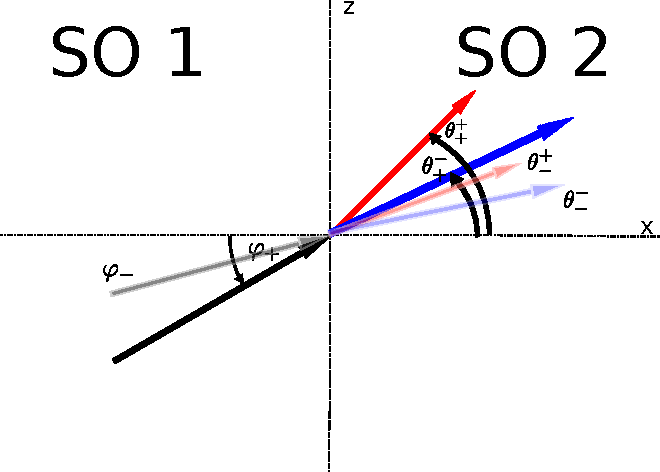
\includegraphics{setup-two-so-regions.pdf}
    \end{center}
    \caption{Scheme of the interface between two regions with
        different, non-zero spin orbit coupling}
    \label{fig:setup-nonzero}
\end{figure}

One just has to remember that the incident beam is split up
into two beams of different chirality, which propagate at different
angles. In general, each beam is split up into two beams at the
interface, so there are up to four beams in \emph{SO B} region,
two of each chirality.

Figure \ref{fig:setup-nonzero} gives an overview of the beams and how
we name them and the associated angles. We will focus our discussion
on the wave with $+$ chirality in the \emph{SO A} region, and the
resulting waves in the \emph{SO B} region.

\begin{figure}
    \begin{center}
        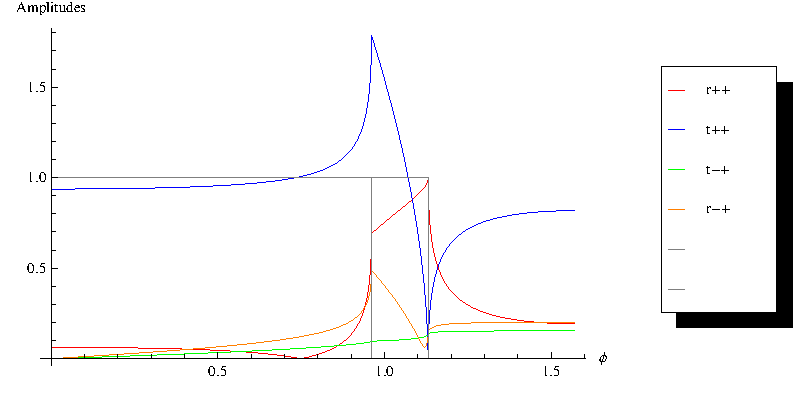
\includegraphics[width=\textwidth]{nonzero-plus.pdf}
        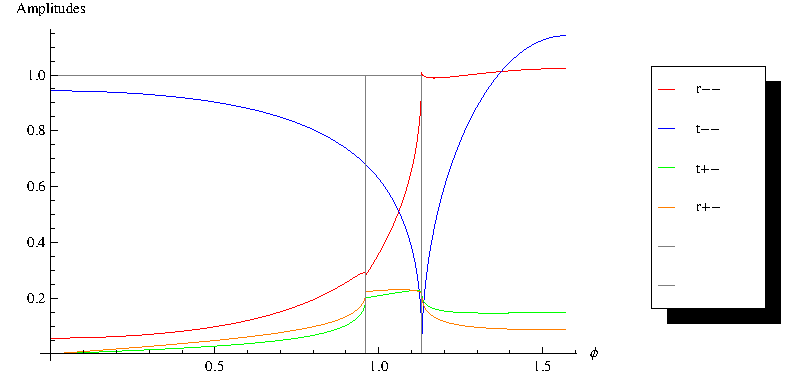
\includegraphics[width=\textwidth]{nonzero-minus.pdf}
    \end{center}
    \caption{Transmission and reflection coefficients for the
        incident $+$ (top) and $-$ (bottom) wave, with
        $\ta_1 = 0.1$ and $\ta_2 = 0.2$.}
    \label{fig:plots-nonzero}
\end{figure}

As before, equations \ref{eq:continuous} and \ref{eq:j_continuous}
apply and can be solved unambiguously. Figure \ref{fig:plots-nonzero}
shows the transmission coefficients as a function of $\phi$ as a
result from these equations.

As before we can identify a critical angle above which the $+$ wave
does not propagate. Instead of using the condition $\theta^+_+ =
\frac{\pi}{2}$ it is easier to look at the momentum directly:

\begin{align}
    p_{x,B}^+ = \sqrt{ p_B^2 - p_z^2} = p \sqrt{(\sqrt{1+\ta_B^2} -
            \ta_B)^2 - \sin^2 \phi^+}
\end{align}

For $p_B^2 < p_z^2$ the mode is evanescent because $p_{x,B}$ is
imaginary. For $p_B^2 = p_z^2$ the angle $\phi^+$ reaches its critical
value, which is only dependent on the strength of the spin-orbit
coupling strength in the right regime:

\begin{align}
    \phi^+_{c1} = -\sin^{-1}(\ta_B - \sqrt{1+\ta_B^2})
\end{align}

This is the first gray vertical line in figure
\ref{fig:plots-nonzero}, and in the region $\phi < \phi+_{B,c}$ the various transmission and reflection
coefficients look very similar to the case with $\ta_A = 0$.

The second gray line is critical angle $\phi^+_{c2}$ associated with
$\ta_A$. For
$\phi > \phi^+_{A,c}$ the momentum in $x$ direction $p_{x,A}$ is again
imaginary, just like if we had another interface to a normal region
left of the $A$ region. 

It follows the same $\ta$ dependency, namely $\phi^+_{c2} =
-\sin^{-1}(\ta_A - \sqrt{1+\ta_A^2})$.

%
%\begin{figure}
%    \begin{center}
%        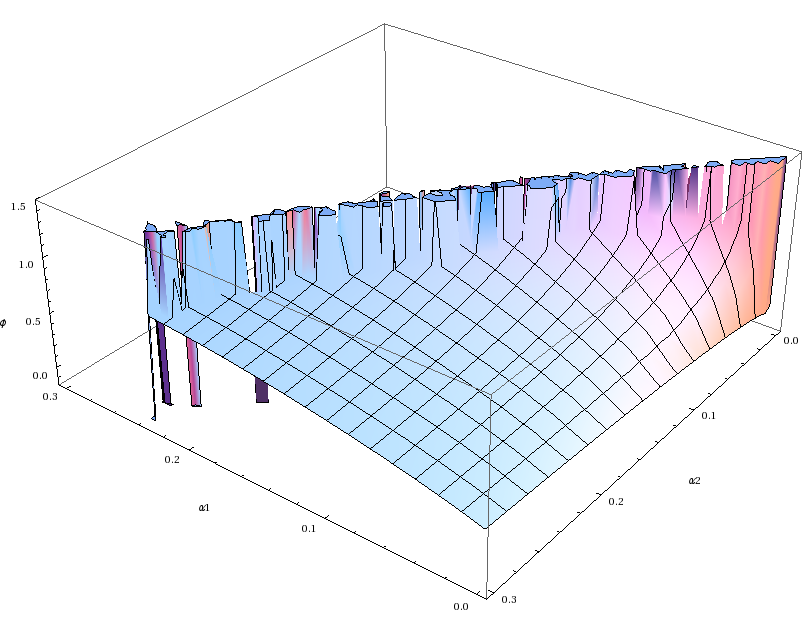
\includegraphics[width=0.8\textwidth]{rpp-zero-point.png}
%    \end{center}
%    \caption{$\phi_0$, the angle for which $r_{++}$ vanishes, as a
%        function of $\ta_1$ and $\ta_2$ (numerically determined)}
%    \label{fig:rpp-zero-point}    
%\end{figure}
%
%For $\ta_2 > \ta_1$ there's a point for which $r_{++}(\phi_0) =
%0$. Figure \ref{fig:rpp-zero-point} shows $\phi_0$ as a function of
%$\ta_1$ and $\ta_2$.

% vim: ts=4 sw=4 expandtab spell spelllang=en_us tw=70
